\chapter{Russian Post Offices in China}  
\subsection{Russian Embassy Post}



\begin{figure}[htbp]
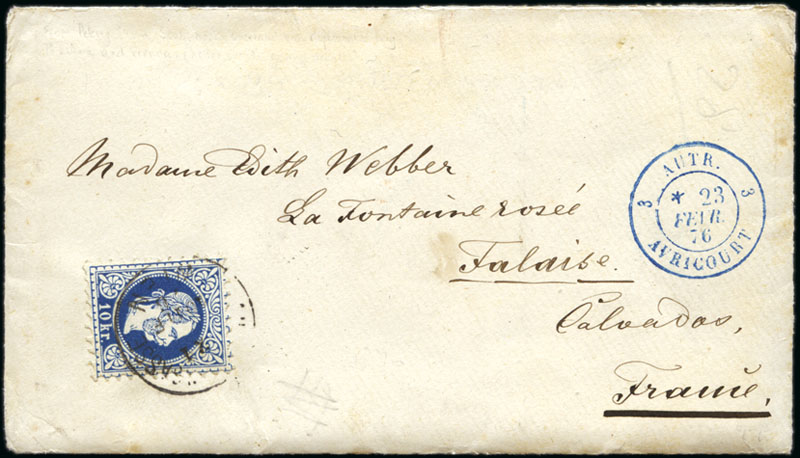
\includegraphics[width=.98\textwidth]{../russian-post-offices-in-china/10002.jpg}
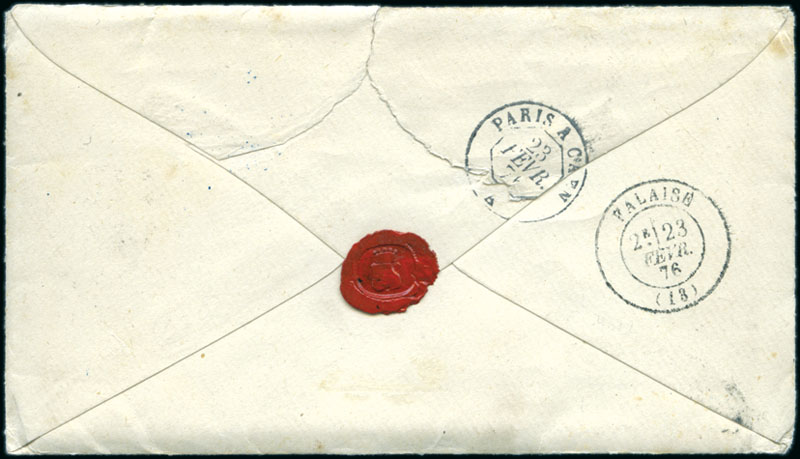
\includegraphics[width=.98\textwidth]{../russian-post-offices-in-china/10002-1.jpg}
\caption{
10002 RUSSIAN EMBASSY IN CHINA POST: 1875 (Dec 16) Cover to France incl. 
contents datelined "Peking, le 16 Dec 1875", carried by the Embassy post 
from Peking through diplomatic channels to St. Petersburg and on to Vienna, 
where it was franked with Austrian 10k and put into the normal post, with 
French transits and reverse with wax nobility seal.
Note: This incredible routing is confirmed by the contents which says: 
"Do not be surprised to see on this letter Viennese postage stamps. 
I am sending in the winter all my packets by the Russian Courier free to 
St. Petersburg and from there they are sent on to Vienna".
Freezing over of the River Yangtze is given as the reason 
for this unusual route for this correspondence. Use of the Diplomatic Bag 
would have been in deference to the sender's status.
Provenance: Ex Beckeman
\euro 4,000.00
}  

\end{figure}







    